\label{chap:07_domain_adaptation}
\newcommand{\deacc}[0]{\textbf{deacc}}
\newcommand{\cased}[0]{\textbf{cased}}
\newcommand{\uncased}[0]{\textbf{uncased}}

En este capítulo exploraremos cómo mejorar la detección de discurso de odio desde una perspectiva más general, mediante \textbf{técnicas de adaptación de dominio} y entrenando modelos de lenguaje en textos sociales. Hemos visto en capítulos anteriores que las técnicas de representación utilizadas en los últimos años (desde los word-embeddings hasta los modelos de lenguajes pre-entrenados) generan, por un lado, representaciones ricas al ser entrenadas en dominios sociales; y, así mismo, también observamos que en algunos modelos pre-entrenados (como AWD-LSTM usando la técnica de ULMFit) \todo{meter citas} continuar el entrenamiento sobre un conjunto de datos similar al de la tarea objetivo ayuda a mejorar la performance.

Los modelos de lenguaje suelen ser entrenados sobre cierto conjunto de datos que se suponen suficientemente generales, como Wikipedia que comprende textos de carácter enciclopédico, o como Common Crawl, que es una recopilación de datos de distintos sitios web\footnote{[\url{https://commoncrawl.org/}]}. El uso del lenguaje en estas fuentes suele tener cierta discordancia con el lenguaje de muchas tareas; por ejemplo, tareas en textos médicos, textos científicos, o --lo que es de interés en esta tesis-- las tareas sobre textos sociales tienen un uso del lenguaje muy particular, con mucha jerga, expresiones particulares, y otros usos que se diferencian de los textos fuentes en los que están entrenados BERT, RoBERTa, \beto{} y otros. A cada uno de estos grupos de textos con cierta relación se los denomina --de manera poco concisa-- \textbf{dominios}, y al conjunto de técnicas utilizadas para adaptar distintos modelos a estos \textbf{adaptación de dominio}.

Teniendo estas consideraciones en cuenta, intentaremos  usando técnicas del estado del arte. En primer lugar, entrenando desde cero un modelo de lenguaje basado en transformers (RoBERTa)\cite{liu2019roberta} sobre tweets, al cual llamamos \robertuito{}; la segunda, tomando un modelo \beto{}, y continuando el pre-entrenamiento sobre un gran conjunto de tweets. Trabajo previo ha demostrado que ambas estrategias mejoran la performance de los modelos de clasificación del estado del arte cuando trabajamos en dominios especializados; sin embargo, ninguna comparación se ha realizado entre estas dos formas de abordar el problema \footnote{O al menos seguro no se hizo en español}. de interés dado el gran costo que tiene por detrás entrenar modelos basados en transformers. Para ello, utilizamos como benchmark de este análisis las tareas que hemos tratado en esta tesis, introducidas en los capítulos \ref{chap:03_social_text_classification}, \ref{chap:04_hate_speech} y \ref{chap:06_contextualized_hate_speech}.

Comenzamos en la sección \ref{sec:domain_adaptation_previous_work} haciendo un racconto de las técnicas de adaptación de dominio y modelos pre-entrenados sobre distintos dominios. En la sección \ref{sec:robertuito_pretrained_model} describimos la construcción y el entrenamiento de \robertuito{}, y en la sección \ref{sec:domain_adaptation_vs_robertuito} describimos la adaptación de dominio de \beto{} al dominio social y comparamos la performance de estos modelos contra \robertuito{}.

\section{Trabajo previo}
\label{sec:domain_adaptation_previous_work}

- Qué es un dominio? Escribir un poco de esto (ver paper de gururangan)

\citet{goodfellow2016deep} define la adaptación de dominio como una situación similar a la de Transfer Learning: dado un modelo que fue entrenado sobre una distribución de datos o dominio $P_1$, lo utilizamos sobre una distribución $P_2$ relativamente similar. Concretamente, nos referimos a la aplicación de alguna técnica que ajuste la distribución de la entrada (de $P_1$) a la distribución de nuestro nuevo dominio (la distribución $P_2$), bajo la asunción de que ambas distribuciones son relativamente similares. \citet{glorot2011domain} es uno de los primeros trabajos que aplica esta técnica en NLP, usando denoising auto-encoders para este fin. \todo{Escribir un poco más de esto}

Para lo que nos concierne en NLP solemos querer, dado un modelo de lenguaje (tanto causal como enmascarado) entrenado en un dominio, ajustarlo a otro dominio distinto. Por ejemplo, un modelo BERT pre-entrenado en textos formales (como Wikipedia o noticias) queremos ajustarlo a la distribución de textos sociales, que si bien ambas mantienen el idioma (inglés o español) suelen tener distribuciones notoriamente distintas.

Dentro de la última ola que sacudió NLP de modelos pre-entrenados, ULMFit \citet{howard-ruder-2018-universal} contempla una etapa de adaptación de dominio utilizando de manera no-supervisada el texto del dataset supervisado de la tarea atacada.

Concretamente, dentro de las tareas de extracción de opiniones en redes sociales --lo que nos concierne en esta tesis-- la adaptación de dominio resulta importante ya que expresiones en distintos ámbitos pueden tener sentidos distintos: citando un ejemplo de \citet{pang2008opinion}, decir ``leé el libro'' en una reseña de un libro Amazon puede ser algo positivo, mientras que en el comentario de una película puede ser considerado negativo.

Recientemente, \citet{gururangan-etal-2020-dont} analizan el impacto de los ajustes de dominio. Para ello, consideran varios dominios como ser biomédico, reviews de películas, papers de cs. de la computación (CS), y noticias. Plantean dos configuraciones de adaptación de dominio:

\begin{itemize}
    \item Domain Adaptation: ajustar el modelo de lenguaje sobre un extenso conjunto de datos no etiquetado, usualmente el ``sobrante'' del proceso de recolección que no es anotado
    \item Task Adaptation: ajustar el modelo de lenguaje sobre el dataset, de la misma manera que se hace en ULM-Fit
\end{itemize}

En todos los casos, usando modelos del estado del arte como RoBERTa muestran que aplicar conjuntamente lo que ellos consideran Domain Adaptation y Task Adaptation mejora la performance significativamente. La adaptación, dado que usan modelos como RoBERTa, consiste tan sólo en correr la tarea de MLM sobre los textos del dominio a adaptar.

\begin{table}
    \centering
    \begin{tabular}{llll}
        Nombre                                 & Idioma            & Dominio                          & Familia     \\
        \hline
        SciBERT\cite{beltagy-etal-2019-scibert} & Inglés            & Papers científicos               & BERT        \\
        BERT-CT                                 &                   &                                  &             \\
        ClinicalBERT\cite{huang2019clinicalbert}& Inglés            &                                  & BERT        \\
        BERTweet\cite{bertweet}                 & Inglés            & Tweets, algunos COVID-related    & RoBERTa     \\
        TwilBERT                                &                   &                                  &             \\
        AlBERTo                                 &                   &                                  &             \\
    \end{tabular}

    \caption{Modelos pre-entrenados sobre distintos dominios. En familia nos referimos a qué tipo de modelo de lenguaje es usado (BERT, RoBERTa, etc)}
    \label{tab:bert_pretrained_models}
\end{table}


Luego del estallido de los modelos de lenguaje basados en transformers, algunos trabajos se han basado en directamente entrenar estos modelos ya no en textos formales como Wikipedia o noticias sino directamente en el dominio en cuestión. Por ejemplo, SciBERT \cite{beltagy-etal-2019-scibert} es un modelo BERT entrenado directamente en textos científicos, BERTweet \cite{bertweet} entrena un modelo RoBERTa\cite{liu2019roberta} sobre cerca de 850M tweets en inglés, una parte de ellos relacionados a la pandemia del COVID-19. La tabla \ref{tab:bert_pretrained_models} lista algunos de estos modelos.

En español tenemos el modelo TwilBERT\cite{gonzalez2021twilbert}; sin embargo, tiene algunas limitaciones: en primer lugar, no queda claro cuánto tiempo de entrenamiento recibió ni si los datos fueron suficientes; en segundo, usaron un modo de entrenamiento basado en una variante de la tarea NSP (ver subsección XXX) cuando numerosos trabajos muestran que el tipo de entrenamiento basado en RoBERTa (sólo tarea MLM) mejora el desempeño. Finalmente, su modelo no es accesible mediante el hub de huggingface\todo{agregar URL o cita}, que usamos para este trabajo.


Algunas oportunidades de mejora de lo estudiado en \citet{gururangan-etal-2020-dont} son, en primer lugar y siguiendo la regla de Bender\cite{bender2011achieving}, realizar el estudio en un idioma distinto del inglés. Por otro lado, un dominio que no está estudiado en dicho trabajo es el dominio de tareas en textos sociales. Finalmente, y dado el estallido dees de interés realizar una comparación de la performance de modelos adaptados al domini

\section{Tareas utilizadas en el benchmark}

Para analizar el impacto de la adaptación de dominio y realizar una comparación contra un modelo entrenado desde cero en dicho dominio usamos un conjunto de tareas como benchmark. Las tareas elegidas son todas las que analizamos en este trabajo hasta el momento:

\begin{enumerate}
    \item Detección de discurso de odio
    \item Detección contextualizada de discurso de odio
    \item Análisis de sentimientos
    \item Análisis de emociones
    \item Detección de Ironía
\end{enumerate}

La única tarea que no estudiamos hasta el momento es la de detección de ironía, que es básicamente una tarea de detección binaria sobre textos sociales para distintos. Todas las tareas (con la excepción de la detección contextualizada explicada en los capítulos anteriores) forman parte de IberLEF.




\section{Modelo pre-entrenado sobre tweets}
\label{sec:robertuito_pretrained_model}

Pasamos a continuación a describir a \robertuito{}, un modelo de lenguaje pre-entrenado sobre tweets en español. Proponemos tres versiones de \robertuito{}: una versión \emph{cased} que conserva las mayúsculas, una versión \emph{uncased} que convierte todo a minúsculas y una versión \deacc{}, que usa minúsculas y elimina los acentos en los tweets. El español usa tildes para enfatizar los acentos en las palabras; por lo general, se pasan por alto en los textos sociales, por lo que queremos analizar si eliminarlos mejora el rendimiento de los modelos.

Entrenamos a los tokenizadores usando el algoritmo \emph{SentencePiece} en los tweets recopilados para cada una de las tres configuraciones. Guardamos 30K tokens para cada uno. Usamos \emph{tokenizers} library \footnote{\url{https://github.com/huggingface/tokenizers}} que proporciona implementaciones rápidas en el lenguaje de programación Rust para muchos algoritmos de tokenización.


\subsection{Recolección de tweets}

A continuación describimos el proceso de recolección de tweets que utilizamos para entrenar \robertuito{}.

El stream de API de acceso gratuito (también conocida como \emph{Spritzer}) es una muestra de alrededor del 1\% de los tweets, supuestamente aleatoria, aunque algunos estudios han mostrado algunas preocupaciones acerca de la posible manipulación de esta muestra \cite{pfeffer2018tampering}. Si bien esto puede ser un problema para estudios de ciencias sociales computacionales, para nuestros fines descartamos estas preocupaciones.

En primer lugar, descargamos una colección de Spritzer subida a Archive.org que data de Mayo de 2019\footnote{\url{https://archive.org/details/archiveteam-twitter-stream-2019-05}}. Filtramos aquellos tweets cuya metadata indique que su idioma no sea español. Sobre los tweets en español, usamos la API de Twitter para descargar los tweets de los usuarios en cuestión. De este proceso recolectamos alrededor de 622 millones de tweets de cerca 432 mil usuarios.

Finalmente, considerando que no queremos entrenar , nos quedamos sólo con aquellos tweets que tengan 6 o más tokens, usando para esto el tokenizador entrenado en BETO \cite{canete2020spanish}, sin contar repeticiones de emojis y haciendo el preprocesado descripto en capítulos anteriores: reemplazamos los caracteres hasta un máximo de tres, convertimos los nombres de usuarios a un token especial \verb|@usuario|, convertimos los emoji a una representación textual, y partimos los hashtag en lo posible (ver sección XXX). Esto lo realizamos a priori para bajar la carga de trabajo a la hora del pre-entrenamiento.

De este proceso quedan 500M tweets, los cuales ordenamos en 1000 archivos para facilitar la lectura en procesos posteriores. El repositorio de la recolección de tweets puede encontrarse en \url{https://github.com/finiteautomata/spritzer-tweets}.


\subsection{Arquitectura y entrenamiento}

\begin{table}[t]
    \centering
    \begin{tabular}{l|l}
        \hline
        Hyperparameter  & Value \\
        \hline
        \#Heads           & 12             \\
        \#Layers          & 12             \\
        Hidden Size       & 768            \\
        Intermediate Size & 3072           \\
        Hidden activation & GeLU           \\
        Vocab. size       & 30,000         \\
        \hline
        MLM probability   & 0.15           \\
        Max Seq length    & 128            \\
        Batch Size        & 4,096          \\
        Learning Rate     & $3.5 * 10^{-4}$\\
        Decay             & $0.1$          \\
        $\beta_1$         & 0.9            \\
        $\beta_2$         & 0.98           \\
        $\epsilon$        & $10^{-6}$      \\
        Warmup steps      & 36,000 (6\%)   \\
        \hline
    \end{tabular}
    \caption{Hiperparámetros utilizados en el entrenamiento de \robertuito{}.}
    \label{tab:robertuito_architecture}
\end{table}

Se utilizó una arquitectura RoBERTa base para \robertuito{}, con 12 capas de auto atención, 12 cabezas de atención y tamaño intermedio 768, de la misma manera que BERTweet \cite{bertweet}. Entrenamos sobre la tarea de MLM, en la misma línea de RoBERTa y BERTweet, sin tener en cuenta la tarea de predicción de la siguiente oración usada en BERT u otras tareas de orden de tweets como la usada en \citet{gonzalez2021twilbert}.

Teniendo en cuenta los hiperparámetros de RoBERTa y BERTweet, decidimos utilizar un tamaño de batch size grande para nuestro entrenamiento. Si bien se recomienda un tamaño de 8k en RoBERTa, debido a las limitaciones de recursos, decidimos equilibrar el número de actualizaciones utilizando un tamaño de lote de 4k.

Para comprobar la convergencia, primero entrenamos un modelo uncased para 200k pasos de optimización. Al comprobar que convergió (y obtuvo buenos resultados en las tareas del benchmark), procedimos al entrenamiento completo de los tres modelos.

Entrenamos nuestros modelos durante aproximadamente tres semanas en una TPU v3-8 y una máquina pre-emptible \emph{e2-standard-16} en GCP. Estas nos fueron provistas por el programa Google TPU Research Cloud. Nuestro código está basado en la biblioteca \emph{huggingface's transformers}\cite{wolf-etal-2020-transformers} y su implementación de \emph{RoBERTa}. Cada tweet está tokenizado y enmascarado dinámicamente con una probabilidad igual a $ 0.15 $. La tabla \ref{tab:training_results} muestra los resultados del entrenamiento en términos de pérdida de entropía cruzada y perplejidad.

\begin{table}[h]
    \centering
    \begin{tabular}{l|l l l|}
        Model   & Train loss & Eval loss   & Eval ppl \\
        \hline
        \cased{}   & 1.864      & 1.753       & 5.772    \\
        \uncased{} & 1.940      & 1.834       & 6.259    \\
        \deacc{}   & 1.951      & 1.826       & 6.209
    \end{tabular}
    \caption{Resultados del entrenamiento para las tres versiones de \robertuito{}. La función de costo utilizada es la entropía cruzada de la tarea de Masked-Language-Modeling, y reportamos también la perplejidad (ppl)}
    \label{tab:training_results}
\end{table}


\subsection{Resultados}


\begin{table}
    \centering
    \footnotesize
    \begin{tabular}{llllllr}
        \toprule
        Modelo             & CHATE             &  HATE             &  SENTIMENT        &  EMOTION          &  IRONY            &     score \\
        beto-uncased       & $0.591 \pm 0.006$ &  $0.757 \pm 0.012$ & $0.649 \pm 0.005$ & $0.521 \pm 0.006$ & $0.702 \pm 0.008$ &  0.6438 \\
        bertin             & $0.557 \pm 0.008$ &  $0.767 \pm 0.005$ & $0.665 \pm 0.003$ & $0.518 \pm 0.012$ & $0.716 \pm 0.008$ &  0.6447 \\
        beto-cased         & $0.582 \pm 0.007$ &  $0.768 \pm 0.012$ & $0.665 \pm 0.004$ & $0.521 \pm 0.012$ & $0.706 \pm 0.007$ &  0.6485 \\
        roberta-bne        & $0.577 \pm 0.004$ &  $0.766 \pm 0.015$ & $0.669 \pm 0.006$ & $0.533 \pm 0.011$ & $0.723 \pm 0.017$ &  0.6536 \\
        \hline
        robertuito-cased   & $0.590 \pm 0.005$ &  $0.790 \pm 0.012$ & $0.701 \pm 0.012$ & $0.519 \pm 0.032$ & $0.719 \pm 0.023$ &  0.6636 \\
        robertuito-deacc   & $0.593 \pm 0.006$ &  $0.798 \pm 0.008$ & $0.702 \pm 0.004$ & $0.543 \pm 0.015$ & $0.740 \pm 0.006$ &  0.6753 \\
        robertuito-uncased & $0.593 \pm 0.004$ &  $0.801 \pm 0.010$ & $0.707 \pm 0.004$ & $0.551 \pm 0.011$ & $0.736 \pm 0.008$ &  0.6776 \\
        \hline
    \end{tabular}
    \caption{Resultados de la evaluación de modelos pre-entrenados y modelos ajustados en dominio para el benchmark de tareas sociales: CHATE es contextualized hate speech, HATE es hate speech detection sobre el dataset de hatEval, SENTIMENT, EMOTION e IRONY son análisis de sentimiento, emociones e ironía sobre los corpus de TASS. El score es el promedio de los scores de todas las tareas.}
    \label{tab:robertuito_evaluation_results}
\end{table}


La tabla \ref{tab:robertuito_evaluation_results} muestra los resultados de la evaluación de los modelos seleccionados para las cuatro tareas de clasificación propuestas. Los resultados se muestran como la media de quince ejecuciones de los experimentos, junto con la desviación estándar. Así mismo, calculamos un \textbf{score} promediando las puntuaciones de cada tarea de forma similar a lo hecho en GLUE. Podemos observar que en la mayoría de los casos, todas las configuraciones de \robertuito{} funcionan significativamente por encima de otros modelos, en particular para las tareas de Discurso de odio y Sentimiento. El único caso donde esto no ocurre es en la tarea de detección de discurso de odio contextualizado, donde si bien hay una mejora, es marginal y poco significativa.

Respecto a la comparación entre los tres modelos, analizamos las diferencias entre estos mediante una prueba de la diferencia de medias. Para ello, realizamos un test de Kruskal-Wallis para las performances de cada tarea. Existen diferencias significativas entre el desempeño de los tres modelos de \robertuito{} ($ H (3) = 6.88, p \ leq 0.05 $ para Discurso de odio, $ H (3) = 9.90 , p <0.01 $ para Análisis de sentimiento, $ H (3) = 11.85, p <0.01 $ para Análisis de emociones, $ H (3) = 11.54, p <0.01 $ para Detección de ironía), no así para la detección de odio contextualizado ($H(3)=3.59, p > 0.15$).

Para verificar las diferencias significativas entre las performances de los tres modelos para las 4 tareas mencionadas, realizamos un análisis post-hoc con un test de Dunn (con corrección de Benjamini-Hochberg). \todo{Mandar tablas a un apéndice}. Exceptuando la tarea de análisis de sentimientos, la versión \emph{cased} muestra siempre diferencias significativas contra las versiones \emph{uncased} o \emph{deacc}. Sin embargo, no se encuentran diferencias significativas entre \emph{uncased} y \emph{deacc}.

Este resultado puede leerse de dos maneras: una, que una normalización más fuerte (remover las tildes) del texto de entrada en español no produce una mejora significativa en el rendimiento de los modelos, y dos, que mantener los acentos en el texto de entrada no es beneficioso ni perjudicial para el rendimiento del modelo.

\begin{figure}
    \centering
    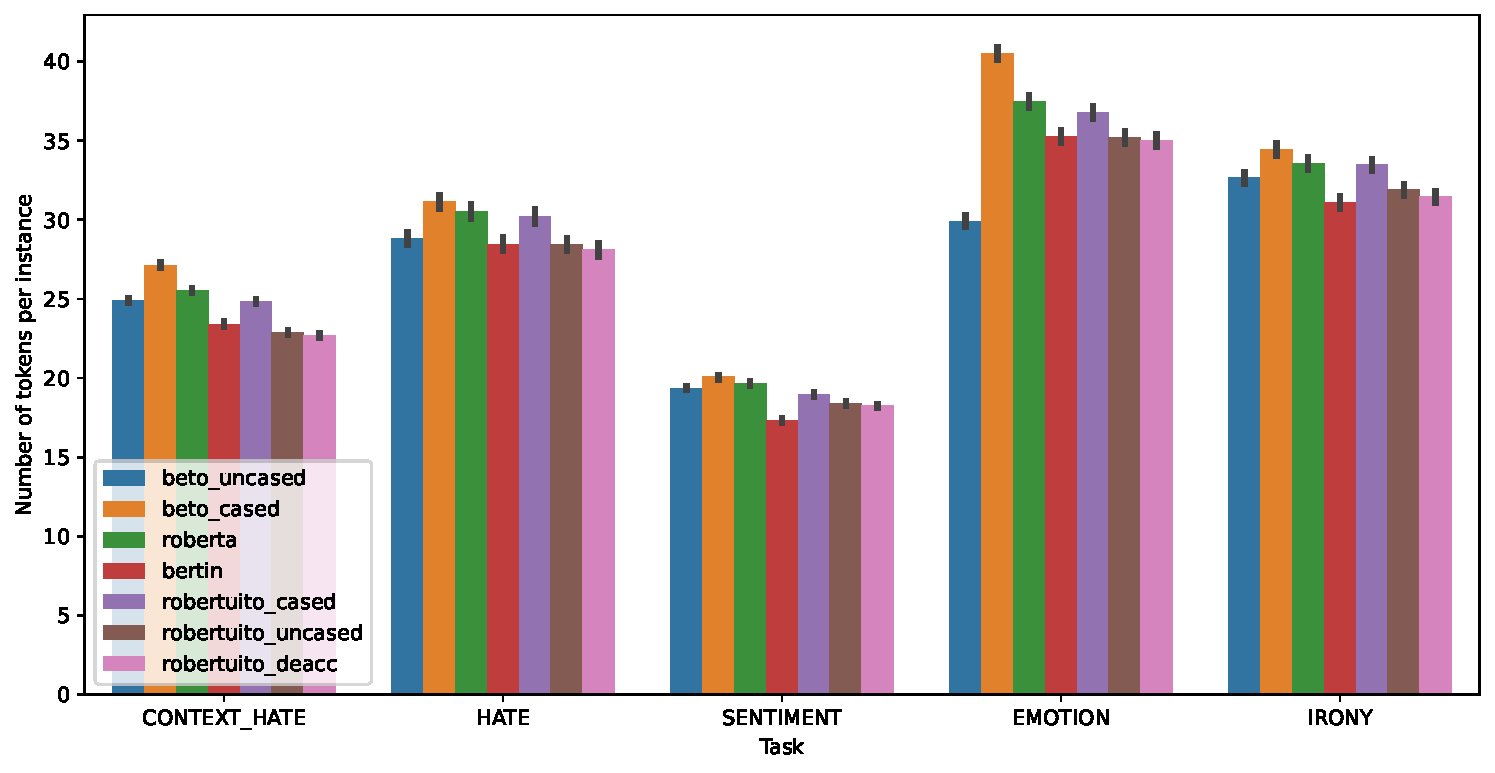
\includegraphics[width=\textwidth]{img/robertuito/length_tokens.pdf}
    \caption{Distribución de la cantidad de tokens por instancia para los tokenizadores de cada modelo. Las barras están agrupadas por tarea y muestran la media de la distribución junto a su intervalo de confianza a 95\%.}
    \label{fig:length_tokens}
\end{figure}

La figura \ref{fig:length_tokens} muestra la distribución del número de tokens en el texto de entrada, agrupados por tarea. Podemos observar que los modelos de \robertuito{} tienen representaciones más compactas que BETO  y \emph {RoBERTa-BNE} ; sin embargo, \emph{bertin} parece tener representaciones iguales o más compactas que él, a pesar de su menor rendimiento en general. Además, entre los modelos de \robertuito{}, podemos observar que la versión \deacc{} tiene una longitud media ligeramente menor en comparación con la versión \uncased{}.


\section{Adaptación de modelos pre-entrenados}
\label{sec:domain_adaptation_vs_robertuito}

Acabamos de observar que \robertuito{} obtiene una mejor performance que otros modelos pre-entrenados. Ahora, ¿puede ser esta mejora replicada adaptando otro modelo de lenguaje? Esta pregunta tiene, más allá del interés teórico de si un modelo de lenguaje entrenado en un dominio distinto puede adaptarse con éxito a un dominio diferente (algo explorado en el trabajo de \citet{gururangan-etal-2020-dont}), tiene dos consideraciones prácticas: en lenguajes de recursos relativamente bajos, entrenar un modelo desde cero como realizamos en la anterior sección puede ser prohibitivo; y por otro lado, reducir los inmensos costos computacionales de entrenar modelos desde cero puede ser de interés.

Para contestar esta pregunta, realizamos una adaptación de dominio a un modelo BETO sobre textos sociales, y probamos su performance sobre el benchmark de tareas sociales descripto en la sección anterior.


\subsection{Metodología}

Para realizar la adaptación de dominio, seguimos las recomendaciones de \citet{gururangan-etal-2020-dont}: tomar un gran conjunto de datos no anotado de textos sociales, y correr la tarea de Masked Language-Modeling sobre estos. En términos de ese trabajo, estaríamos realizando \emph{Domain Adaptation Pre-training} (\emph{DAPT}). Para ello, utilizamos los mismos datos recolectados para entrenar a \robertuito{}.

Tomamos las versiones cased y uncased de BETO, y corrimos únicamente la tarea de MLM sobre estos datos. En lugar de correr por 12.5K pasos de optimización como es sugerido en este trabajo, probamos con 2.5K, 5K, 10K y 20K pasos de optimización, para analizar también el impacto de este hiperparámetro. Finalmente, nos quedamos con la configuración que obtuvo el mejor resultado en términos del benchmark analizado.

Para entrenar estos modelos, usamos una TPU v2-8, gracias también al programa TRC de Google. Cada paso de optimización tomó alrededor de 2.5 segundos. Usamos una configuración similar a la descripta para el entrenamiento de \robertuito{} (ver tabla \ref{tab:robertuito_architecture}), con un learning rate levemente superior ($5 * 10^-4$) y limitando también la longitud de secuencia a 128 tokens.

\subsection{Resultados}
\label{sec:domain_adaptation_results}


\begin{figure}
    \centering
    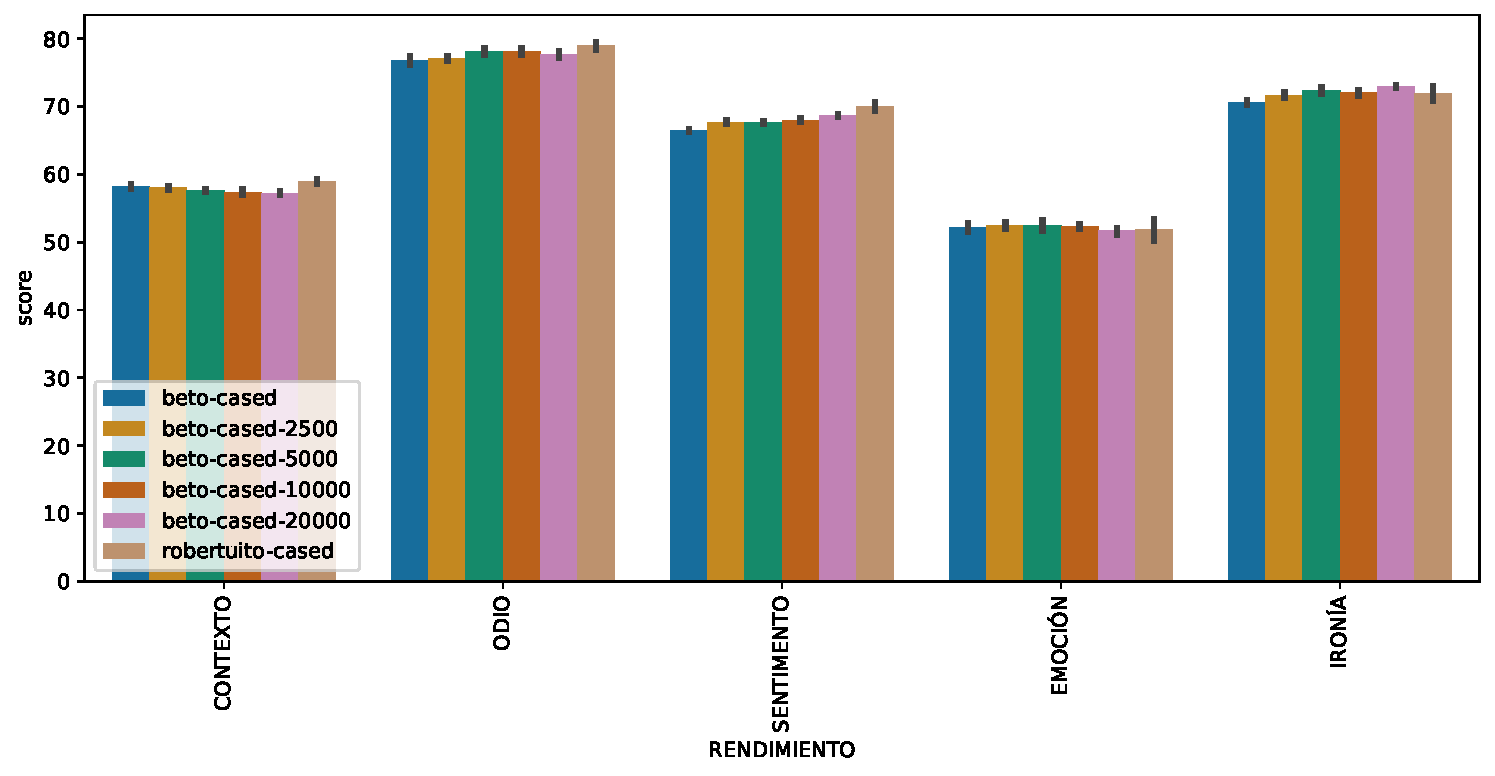
\includegraphics[width=\textwidth]{img/robertuito/results_cased_models.pdf}
    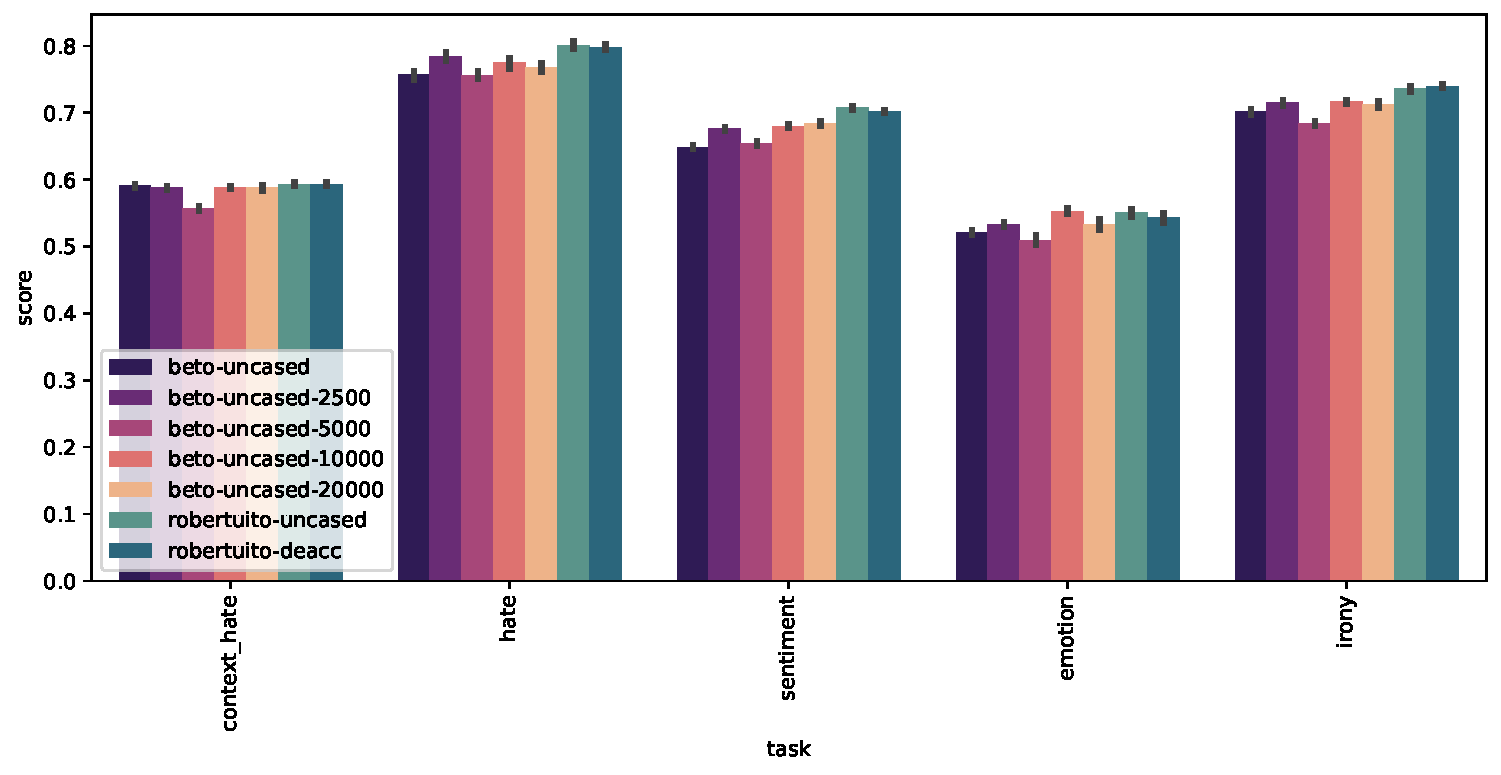
\includegraphics[width=\textwidth]{img/robertuito/results_uncased_models.pdf}

    \caption{Resultados sobre el benchmark de los modelos BETO y \robertuito{} (en versiones cased y uncased). Las barras están agrupadas por tarea y muestran la media de la performance sobre 15 corridas, junto a su intervalo 95\%. En tonalidad de rojo oscuro a amarillo están los modelos ajustados a dominio (más claro, más ajuste de dominio). En tonos azules las variantes de \robertuito{}}
    \label{fig:robertuito_vs_domain_barplot_results}
\end{figure}


En la figura \ref{fig:robertuito_vs_domain_barplot_results} podemos observar la performance para los modelos de lenguaje (\beto{} y \robertuito{}) así como también para las versiones con ajuste de dominio de \beto{}. Marcamos, por ejemplo, \emph{beto-cased-5000} a aquel modelo \beto{} ajustado a dominio por 5,000 pasos de optimización. Podemos observar que, para los modelos \emph{cased}, aumentar el pre-entrenamiento pareciera coincidir con una mejor performance; salvo para el caso de la tarea de detección de odio contextualizado. Una posible razón detrás de esto es que la tarea planteada en esta tesis tiene diferencias con el dominio sobre el cual ajustamos: utilizamos pares de tweets, uno de ellos (el contexto) proveniente de un medio periodístico.

En el caso de los modelos \emph{uncased}, esta mejora es un poco menos clara: por ejemplo, podemos observar que a los 5,000 pasos de optimización la performance sufre una caída con respecto a otras tareas. Esto puede deberse a problemas en la recolección de datos en los cuales entrenamos \robertuito{}, que se magnifican al realizar pocas actualizaciones. Sin embargo, salvando este caso puntual, observamos mejoras en todas las tareas, otra vez salvando el caso de la detección de odio contextualizada.

La tabla \ref{tab:domain_adaptation_evaluation_results} muestra las medias de los resultados junto a sus desviaciones estándar para los modelos \emph{uncased}, que tienen los mejores resultados (ver en apéndice ZZZZ la tabla completa). Seleccionamos como modelos ajustados a dominio



\begin{table}[ht]
    \centering
    \footnotesize
    \begin{tabular}{llllllr}
        \toprule
        Modelo             & CHATE                   &  HATE              &  SENTIMENT        &  EMOTION          &  IRONY            &     score \\
        \midrule
        beto-uncased       & $0.591 \pm 0.006$ & $0.757 \pm 0.012$ & $0.649 \pm 0.005$ & $0.521 \pm 0.006$& $0.702 \pm 0.008$& 0.644 \\
%       bertin             & $0.557 \pm 0.008$ & $0.767 \pm 0.005$ & $0.665 \pm 0.003$ & $0.518 \pm 0.012$& $0.716 \pm 0.008$& 0.644702 \\
        beto-cased         & $0.582 \pm 0.007$ & $0.768 \pm 0.012$ & $0.665 \pm 0.004$ & $0.521 \pm 0.012$& $0.706 \pm 0.007$& 0.648 \\
%       roberta-bne        & $0.577 \pm 0.004$ & $0.766 \pm 0.015$ & $0.669 \pm 0.006$ & $0.533 \pm 0.011$& $0.723 \pm 0.017$& 0.653565 \\
        beto-cased$_{FT}$   & $0.572 \pm 0.006$ & $0.777 \pm 0.009$ & $0.686 \pm 0.005$ & $0.517 \pm 0.009$& $0.730 \pm 0.004$& 0.656 \\
        beto-uncased$_{FT}$ & $0.588 \pm 0.003$ & $0.775 \pm 0.015$ & $0.680 \pm 0.004$ & $0.553 \pm 0.009$& $0.717 \pm 0.005$& 0.663 \\
        \hline
        robertuito-cased   & $0.590 \pm 0.005$ & $0.790 \pm 0.012$ & $0.701 \pm 0.012$ & $0.519 \pm 0.032$& $0.719 \pm 0.023$& 0.665 \\
        robertuito-deacc   & $0.593 \pm 0.006$ & $0.798 \pm 0.008$ & $0.702 \pm 0.004$ & $0.543 \pm 0.015$& $0.740 \pm 0.006$& 0.675 \\
        robertuito-uncased & $0.593 \pm 0.004$ & $0.801 \pm 0.010$ & $0.707 \pm 0.004$ & $0.551 \pm 0.011$& $0.736 \pm 0.008$& 0.678 \\
        \bottomrule
    \end{tabular}
    \caption{Resultados de la evaluación de modelos pre-entrenados y modelos ajustados en dominio para el benchmark de tareas sociales: CHATE es contextualized hate speech, HATE es hate speech detection sobre el dataset de hatEval, SENTIMENT, EMOTION e IRONY son análisis de sentimiento, emociones e ironía sobre los corpus de TASS. Todos los scores son Macro F1s. beto-cased-ft y beto-uncased-ft son modelos adaptados al dominio sociall. Score es la media de cada fila. Gap es.. delta es...}

    \label{tab:domain_adaptation_evaluation_results}

\end{table}


\section{Discusión}

Podemos observar que \robertuito{} presenta mejoras significativas para casi todas las tareas, con picos de hasta casi 4 puntos de F1 para la tarea de Sentiment Analysis. La mejora es muy marginal en el caso de la tarea del dataset construído en el capítulo \ref{chap:05_dataset_creation}, y no pareciera ser significativa. Esto puede deberse a que este dataset tiene una estructura bastante diferente de la de las otras tareas: cada instancia es una composición de dos tweets, uno de los cuales (el contexto) es en la mayoría de los casos un titular de diarios (formulado como un tweet), y por otro lado el comentario efectivo que se analiza como discurso de odio. Esto puede mitigar las potenciales mejoras de \robertuito{} por dos razones: el dominio del contexto no es demasiado distinto que el dominio de entrenamiento de BETO, y el tipo de pre-entrenamiento sólo con MLM y no en pares de tweets (recordemos que sólo hacemos MLM y no Next-Sentence Prediction). Sobre la segunda posible razón, podemos observar (para la tarea de detección de discurso de odio contextualizado) que los modelos con pre-entrenamiento basado en RoBERTa (\emph{roberta-bne} y \emph{bertin}) tienen peor performance que las dos versiones de \emph{BETO}.

De los distintos tipos de normalización de texto utilizados en \robertuito{} (\emph{cased}, \emph{uncased} y \emph{deacc}), podemos observar que los modelos \emph{uncased} y \emph{deacc} obtienen mejores performances en general. Si bien el modelo \emph{uncased} muestra una ligera performance superior al modelo \emph{deacc}, esta mejora no es significativa. Esto puede indicar que remover tildes no reporta una degradación de la performance. Esto es esperable ya que usualmente no se utiliza esta marcación en el español ``vulgar'' utilizado en las redes sociales. Sin embargo, para llegar a esta conclusión sería necesario realizar pruebas más extensivas sobre otras tareas.

Con respecto a los experimentos de adaptación de dominio, podemos observar que adaptando BETO obtenemos una mejora en todos las tareas contra la versión no ajustada. Comparado con \robertuito{}, las versiones a las que les realizamos fine-tuning logran alrededor del 50\% del performance gap entre \robertuito{} y BETO. Esta comparación, sin embargo, no es del todo justa ya que BETO fue entrenado de una manera distinta que \robertuito{}. Por cuestiones de tiempo no pudieron ser realizados sobre \emph{roberta-bne}(principalmente, ya que éste modelo y \emph{bertin} fueron lanzados mientras hacíamos estos experimentos) pero debería esto ser verificado en el futuro. Puede que este gap sea reducido aún más partiendo desde este otro modelo, y analizando algunas otras opciones que no tratamos en este capítulo: por ejemplo, agregar vocabulario en el ajuste de dominio, algo que por ejemplo fastAi realiza en su implementación de ULM-FIT.

Una consideración práctica de la adaptación de dominio es que permite, en lugar de realizar un costo pre-entrenamiento desde cero (como en el caso de MedBERT y SciBERT que ya relatamos anteriormente), mejorar la performance de un modelo de lenguaje ya entrenado de una manera relativamente económica. En términos concretos, un ajuste de dominio puede realizarse utilizando una placa de GPU en uno o dos días de entrenamiento, mientras que pre-entrenar un modelo desde cero requiere acceso a un hardware más oneroso. Algunos trabajos recientes \cite{izsak2021train} muestran alternativas para hacer esto con recursos reducidos ajustando varios hiperparámetros y usando algunas técnicas de optimización reciente (como LAMB \cite{you2019large}); sin embargo, muchos de estos setups están lejos del alcance de los recursos disponibles de muchos laboratorios. En este escenario, aplicar una optimización de dominio aparece como una alternativa mucho más factible.

Una de las limitaciones de lo estudiado es que \robertuito{} fue entrenado sólo por 600k pasos de optimización, contra los casi 900k pasos de BETO, y los 1M de BERTweet. Hay que observar, que la optimización de BETO se da con un batch size menor (512 vs 4k que usa \robertuito{}) y la de BERTweet se hace un batch size mayor (7k). En el caso de los modelos basados en RoBERTa en español, no tenemos disponible esa información. Con lo cual, esta comparación no es totalmente justa. Otra limitación es la escasa disponibilidad de tareas en español para textos sociales por fuera de clasificación: en \citet{bertweet}, por ejemplo, se estudian también problemas de POS tagging y de NER para textos sociales en inglés.

\section{Conclusiones}

En este capítulo, hemos abordado la tarea de mejorar la performance de la detección de discurso de odio para las tareas planteadas en esta tesis y en el contexto más general de tareas de clasificación sobre textos sociales en español. Para ello, utilizamos como benchmark varias de las tareas que vimos en esta tesis: detección de discurso de odio (en sus dos versiones, no contextualizada y contextualizada), análisis de sentimiento, análisis de emociones, y detección de ironía.

En primer lugar, y en la corriente de modelos pre-entrenados sobre distintos dominios, generamos un nuevo y valioso recurso para la clasificación de textos sociales: \robertuito{}, un modelo de lenguaje basado en \roberta{} sobre tweets en español. Para ello, recolectamos una gran base de datos de tweets en español, y utilizando las TPU provistas por Google realizamos el pre-entrenamiento de este modelo. Los experimentos de clasificación sobre el benchmark arrojaron que \robertuito{} obtiene mejores significativas sobre otros modelos en español. Así mismo, observamos que remover tildes en el preprocesado no reporta una degradación significativa en la performance.

Por otro lado, exploramos un ajuste de dominio sobre modelos actuales para comparar la ganancia de performance y compararla contra \robertuito{}. Para ello, tomamos los modelos de \beto{} (en sus versiones cased y uncased) y corrimos la tarea de MLM sobre los tweets recolectados para entrenar nuestro modelo anterior. Si bien la performance de estos modelos ajustados mejora con respecto de \beto{}, se mantiene por debajo de \robertuito{}. De todas formas, este análisis puede ser de consideración para aquellos lenguajes con menos recursos que no pueden entrenar modelos de lenguaje desde cero. Resta como trabajo futuro realizar estos experimentos sobre más tareas más ricas que no sean exclusivamente de clasificación, y realizar los ajustes sobre los modelos \roberta{} en español para hacer una comparación más justa.

Todos estos experimentos han sido realizados en español. Publicamos tanto el modelo \robertuito{}(\footnote{\url{https://huggingface.co/finiteautomata/robertuito-base-uncased}}), el código para entrenarlo y para correr el benchmark con otros modelos pre-entrenados \footnote{Ambos en  \footnote{\url{https://github.com/pysentimiento/robertuito}}. Una pequeña observación es el que el código de entrenamiento es una adaptación de los ejemplos de huggingface/transformers, ya que la inmensa cantidad de datos que manejamos(cerca de 500gb) no es manejada adecuadamente por la librería huggingface/datasets. Dejamos a quien esté interesado esta aclaración para adaptarla cuando este problema sea resuelto}, y la base de datos de tweets en español.
